\documentclass[../main.tex]{subfiles}

\begin{document}

    O programa a ser simulado aparece descrito no código Assembly abaixo:
	%preparando para adicionar o programa em assembly
	\lstset{ 
			language={[x86masm]Assembler},
			basicstyle=\footnotesize,
			numberstyle=\tiny,
			numbers=left,
			commentstyle=\color{mygreen},
			keywordstyle=\color{blue},
			morekeywords={LI,SWP,ADD,MUL,HALT,STA,LDA,BLT},
			stringstyle=\color{mymauve},
			stepnumber=5,
			numbersep=5pt, %separacao do numero para o codigo
			backgroundcolor=\color{white},
			frame=single,
			captionpos=t, %posicao da legenda do codigo			
	}
	\lstinputlisting{cap/programa.asm}

	Apenas para fins de teste das funções implementadas, o algoritmo carrega o valor 0 na memória RAM (endereço 16), executa operações matemáticas
	com os operadores A e B e decrementa o resultado final destas operações até que este valor seja inferior ao valor gravado na posição de memória 16 da RAM,
	quando isto acontece, o processamento entra em suspensão (\textit{HALT}).
	
	O arquivo de inicialização \textit{ROM\_mem.mif} que contém o programa descrito pode ser visto abaixo:
	
	\lstset{ 			
			basicstyle=\footnotesize,
			numberstyle=\tiny,
			numbers=left,
			commentstyle=\color{mygreen},
			morecomment=[f]{\%},
			keywordstyle=\color{blue},
			morekeywords={WIDTH,DEPTH,ADRESS_RADIX,DATA_RADIX},
			stringstyle=\color{mymauve},
			stepnumber=5,
			numbersep=5pt, %separacao do numero para o codigo
			backgroundcolor=\color{white},
			frame=single,
			captionpos=t, %posicao da legenda do codigo			
	}
	\lstinputlisting{cap/ROM_mem.mif}
	
	O resultado simulado do programa pode ser observado nas figuras~\ref{fig:sim1},~\ref{fig:sim2} e~\ref{fig:sim3},
	onde é possível conferir que o valor dos registradores segue o esperado pelo programa, bem como o comportamento de PC
	e o fluxo do programa sendo alterado pela instrução \textit{BLT}.
	É possível também acompanhar o estado em que se encontra o processador em cada instrução.
	
	\begin{figure}[h]
		\centering
		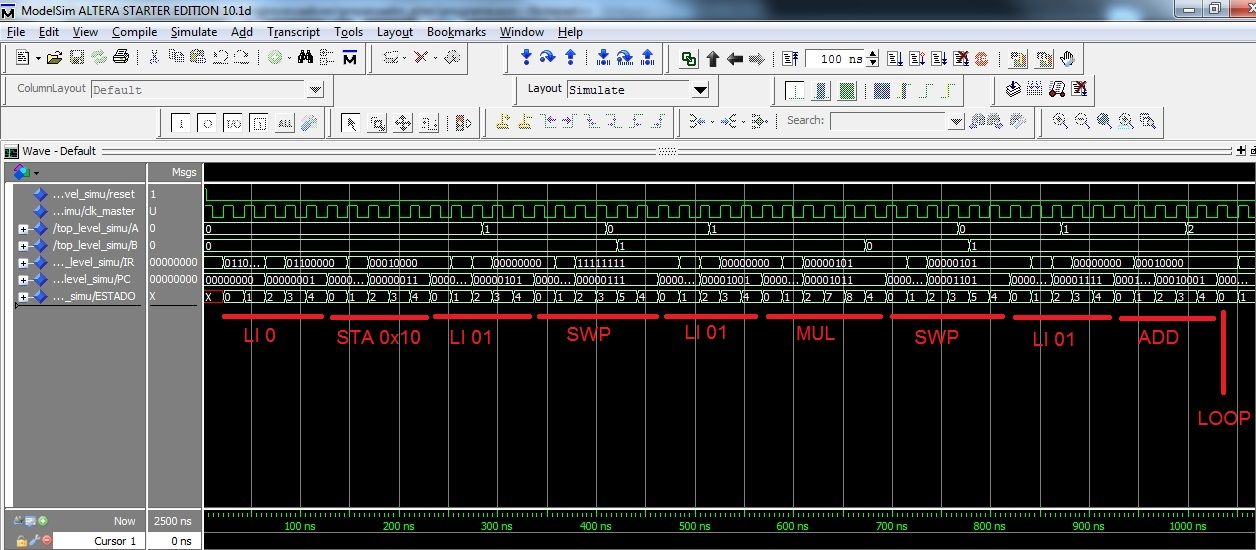
\includegraphics[width=\textwidth]{img/programa_p1}
		\caption{Primeira parte da simulação do programa}
		\label{fig:sim1}
	\end{figure}
		
	\begin{figure}[h]
		\centering
		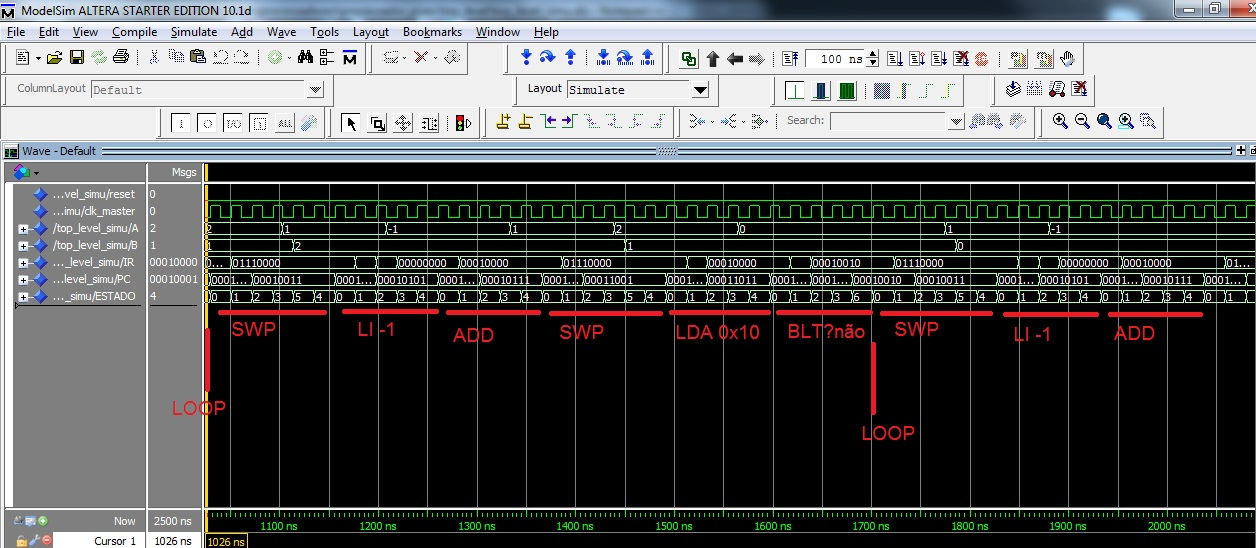
\includegraphics[width=\textwidth]{img/programa_p2}
		\caption{Segunda parte da simulação do programa}
		\label{fig:sim2}
	\end{figure}
		
	\begin{figure}[h]
		\centering
		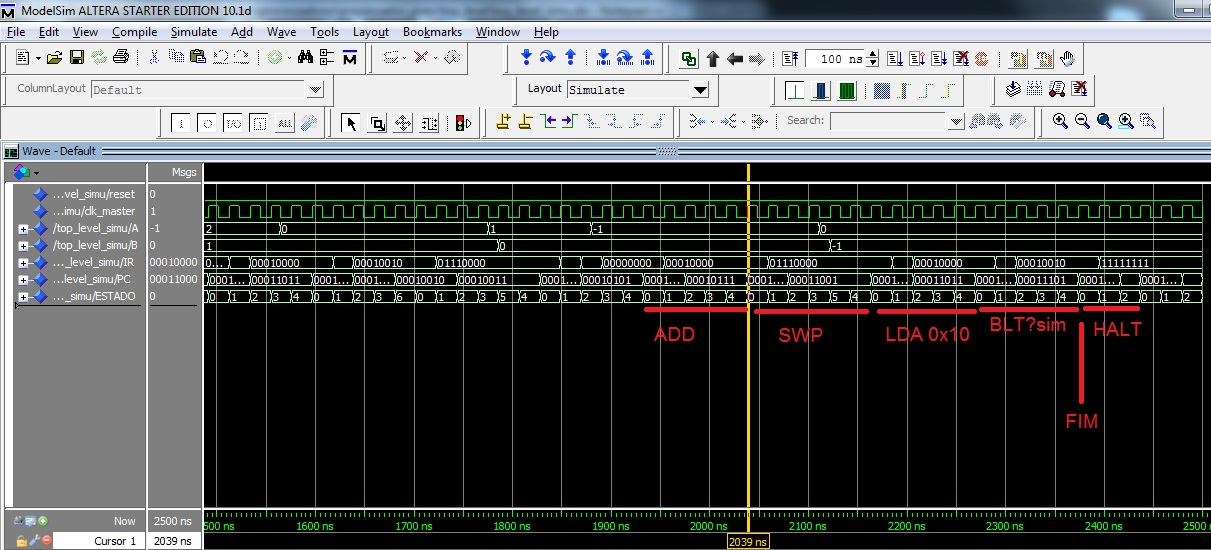
\includegraphics[width=\textwidth]{img/programa_p3}
		\caption{Terceira parte da simulação do programa}
		\label{fig:sim3}
	\end{figure}
\end{document}